\chapter{Results}

\section{Simulated data}

VISOR simulations generated a total of 14 TB of simulated ONT long-read 
sequencing data. Of this volume, approximately 5.6 TB corresponded to reference 
genome-aligned reads in BAM format and their respective indices, while the 
remaining data volume consisted of unaligned reads in FASTQ format 
(\textbf{Table~\ref{tab:file_sizes}}). The computational resources required for 
the simulation process were monitored, with CPU utilization, RAM consumption, 
and generation times detailed in \textbf{Figure~\ref{fig:hpc_visor_laser}}.

\begin{figure}[H]
    \centering
    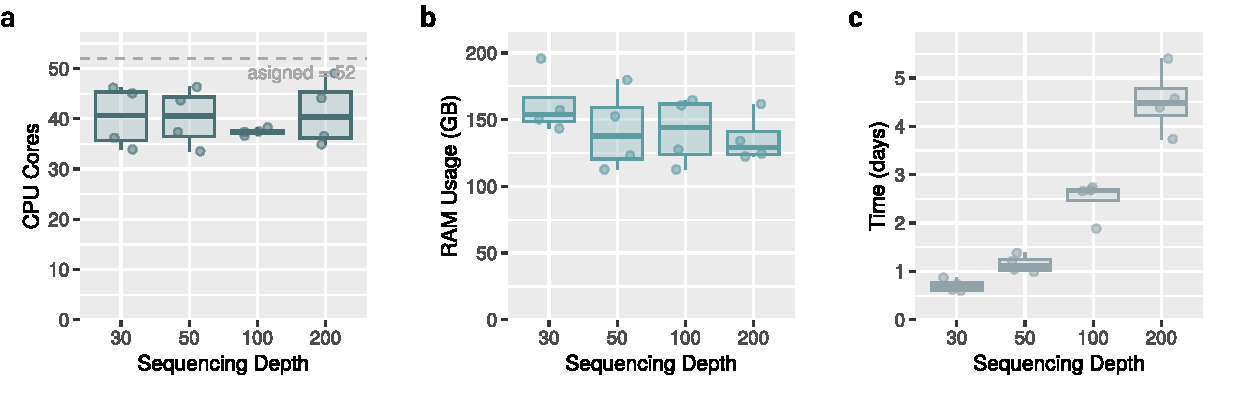
\includegraphics[width=\textwidth]{data/cluster_bmk/hpc_visor_laser.pdf}
    \caption[Computational resources demand of VISOR LASeR module]{Computational 
    resources demand of VISOR LASeR module by sequencing depth, which represents 
    the simulation bottleneck due to its CPU cores (\textbf{a}) and RAM memory 
    (\textbf{b}) consumption over time (\textbf{c}). For each sequncing deph, 
    three ``tumour'' and one ``normal'' WGS technical replicas were obtained 
    by simulating long reads. Calculations for VISOR HACk module were not 
    performed since it runs only once for a few minutes with low resource 
    consumption to introduce the SV set into the reference genome that will 
    feed VISOR LASeR. The raw data used for all calculations is available in REPO.}
    \label{fig:hpc_visor_laser}
\end{figure}

\section{SV calling}

SV callers generate VCF files similar to those produced by SNV callers. However, 
in SV calling, each row represents a breakpoint, which defines the boundary of a 
structural variant. Simple SVs, such as insertions or deletions, require the 
identification of two breakpoints, while complex variants like reciprocal 
translocations necessitate the detection of four breakpoints. To illustrate the 
final output files generated by each caller, results from a 50x coverage 
simulated sample are available at 
\url{https://github.com/villena-francis/master_thesis/tree/main/data/vcf_examples}.

\subsubsection{Standard VCF Outputs}

\begin{itemize}

\item \textbf{SAVANA}. A significant limitation in SAVANA's VCF output, compared 
to other variant callers, is its inability to classify SV types. The tool only 
identifies and correlates breakpoints without providing information about the 
specific type of SV present. 

\item \textbf{Severus}. Beyond conventional SV detection, 
Severus incorporates specialized processing for variable number tandem repeats 
(VNTRs), enabling precise annotation of structural variants within these regions. 
The tool provides comprehensive output including standard VCF files, detailed 
quality metrics in log files, and graphical representations of chromosomal 
rearrangements through visualization plots.

\item \textbf{Sniffles2}. This caller generates standard VCF output exclusively, 
without additional supporting files or visualizations.

\item \textbf{SVision-pro}: Despite leveraging an innovative image-based 
encoding approach to analyze genomic features and detect inter-genome variations 
between tumor-normal paired samples, SVision-pro's output is limited to standard 
VCF files. The visual representations used in its internal processing pipeline 
are not accessible in the final output.

\end{itemize}

\subsection{Computational demands}

While computational requirements for analyzing real samples may be higher due to 
the larger number of SVs typically detected in actual cancer genomes, our 
simulation-based analysis provides proportional estimates of computational 
demands across different sequencing coverages for each of the four callers 
evaluated. Core utilization, RAM consumption, and execution times are 
illustrated in \textbf{Figure~\ref{fig:hpc_calls}}.

A key distinction in processing unit allocation lies with SVision-pro, whose 
neural network-based SV detection model is GPU-optimized, whereas SAVANA, 
Severus, and Sniffles2 rely on CPU-based computation. We allocated 24 cores to 
GPU-based callers, as preliminary testing showed peak utilization remained 
below 20 cores.

The initial RAM allocation of 40 GB proved sufficient for Severus, Sniffles2, 
and SVision-pro, with memory usage increasing linearly with sequencing depth. 
However, SAVANA consistently exceeded this limit across all 
sequencing coverages, demonstrating significantly higher memory requirements 
compared to other callers.

SVision-pro demonstrates the lowest execution times across all sequencing 
depths, followed closely by Sniffles2. Both callers show efficient performance 
scaling, with execution times increasing sub-linearly with sequencing depth. 
SAVANA shows the highest execution times at the three lower sequencing 
coverages (30x, 50x and 100x), while Severus requires the longest processing 
time at maximum coverage (200x).

\begin{figure}[H]
    \centering
    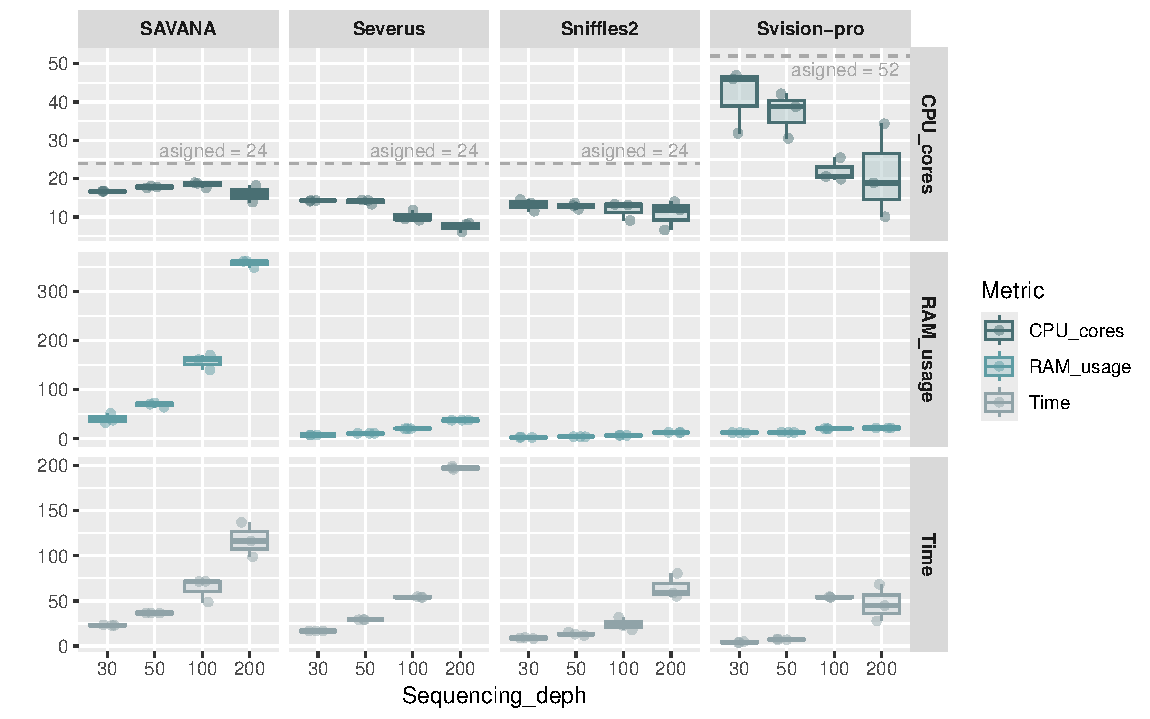
\includegraphics[width=\textwidth]{data/cluster_bmk/hpc_calls.pdf}
    \caption[Computational resource demanded for SV detection methods]{
    Computational resources demanded for SV detection methods of SAVANA, 
    Severus, Sniffles2, and SVision-pro, measured in CPU cores, RAM memory (GB), 
    and execution time (minutes). For each sequencing depth, three measurements 
    per metric were obtained by comparing a single normal sample against three
    technical replicates of the tumor sample. The complete raw data used for
    all calculations is available in 
    \url{https://github.com/villena-francis/master_thesis/tree/main/data/cluster_bmk/hpc_data}.}
    \label{fig:hpc_calls}
\end{figure}

\subsection{Calling performance}

From the proposed SVs in synthetic data, SAVANA and Severus successfully identified 
all instances of tandem duplication, deletion, inversion, and reciprocal 
translocation. Although cut-paste and copy-paste translocations were included in 
the simulation instructions, only the deletion component of cut-paste events was 
successfully reconstructed in the BAM files, while the translocation component and 
copy-paste events failed to be reconstructed.In contrast, neither Sniffles2 nor 
SVision-pro detected any of the simulated SVs, explaining the stark differences 
in Precision, Recall, and F1 scores shown in \textbf{Figure~\ref{fig:perform_calls}}. 


Visual inspection through GW of VISOR-generated BED files confirmed the presence 
of SVs detected by SAVANA and Severus, while validating the absence of 
undetected variants. This verification ruled out false negatives, resulting in a 
recall of 1.0 for both callers. Notably, Severus reported additional findings 
from its specialized VNTR analysis, which, although not explicitly introduced in 
simulation instructions, were present as artifacts from VISOR-LASeR's error 
model.

While SAVANA and Severus achieved identical recall values, SAVANA demonstrates 
higher precision due to Severus reporting slightly more false positives. Despite 
generating significantly more variant calls than both SAVANA and Severus, 
neither Sniffles2 nor SVision-pro detected any of the expected simulated SVs. 
Extensive visual inspection of their findings revealed no overlap with validated 
variants, resulting in their classification as false positives and consequently 
zero precision scores.

As a balanced measure combining precision and recall, F1 score reflects the 
overall performance of each caller. SAVANA achieves the highest F1 score due to 
its perfect recall and superior precision. Severus follows closely, with its 
slightly lower F1 score attributed solely to its marginally higher false 
positive rate, as it maintained perfect recall. Both Sniffles2 and SVision-pro 
yield F1 scores of zero, as expected from their complete absence of true 
positive findings and high number of false positive calls.

\begin{figure}[H]
    \centering
    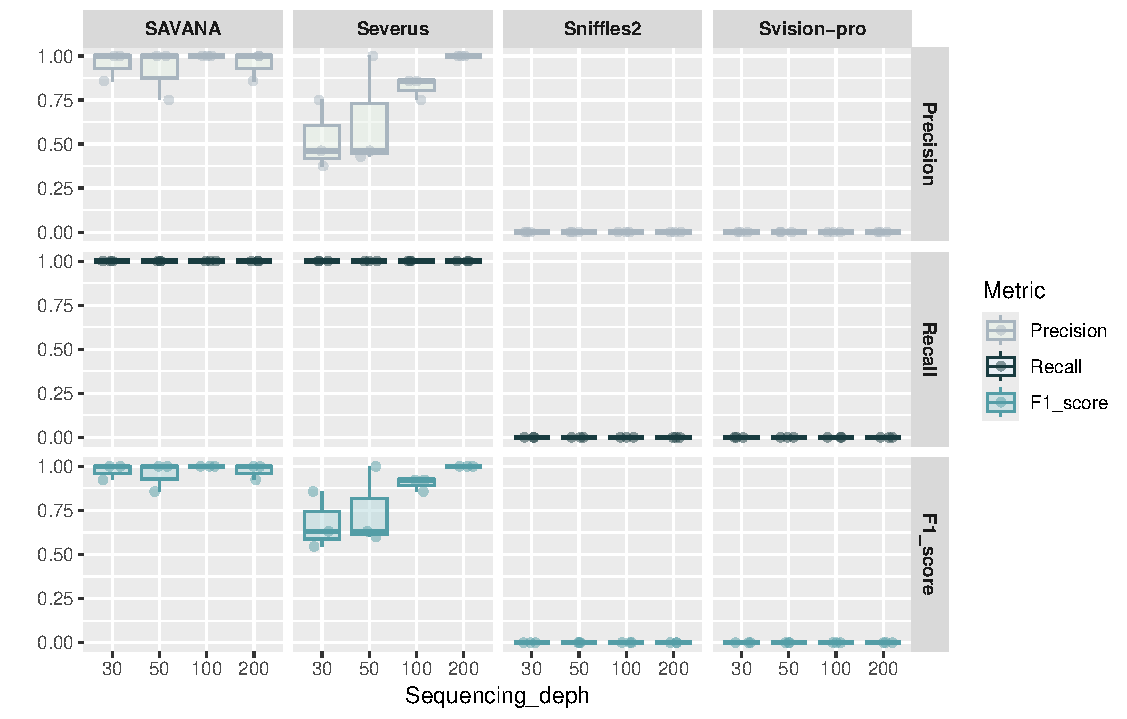
\includegraphics[width=\textwidth]{data/cluster_bmk/perform_calls.pdf}
    \caption[Performance of evaluated SV calling methods]{Performance of SV calling
    methods of SAVANA, Severus, Sniffles2 and SVision-pro, based on precision, 
    recall, and F1 score metrics. For each sequencing depth, three results per 
    metric were obtained by comparing one normal sample against three technical 
    replicates of the tumor sample. The raw data used for all calculations is 
    available in 
    \url{https://github.com/villena-francis/master_thesis/tree/main/data/cluster_bmk/calls_data}.}
    \label{fig:perform_calls}
\end{figure}